\section{Results and Discussion}
\label{sec:results}

% ============================================================
% A. MIXED + SOURCE-DISJOINT
% ============================================================

\subsection{Mixed and Source-Disjoint Performance}

The CustomCNN obtains a mixed Macro-F1 of 0.9453, while the
MobileNetV2 pipeline obtains 0.9775.


\begin{table}[t]
\centering
\caption{Mixed and Source-Disjoint Three-Class Macro-F1}
\label{tab:mixed_source}
\begin{tabular}{lcc}
\hline
Evaluation & CustomCNN & MobileNetV2 \\
\hline
Mixed random & 0.9453 & 0.9775 \\
SD1 & 0.3390 & 0.5274 \\
SD2 & 0.7836 & 0.8514 \\
SD3 & 0.5941 & 0.6942 \\
SD4 & 0.9149 & 0.9175 \\
\textbf{SD1--SD4 mean} & \textbf{0.6579} & \textbf{0.7476} \\
\hline
\end{tabular}
\end{table}


\begin{figure*}[!t]
\centering
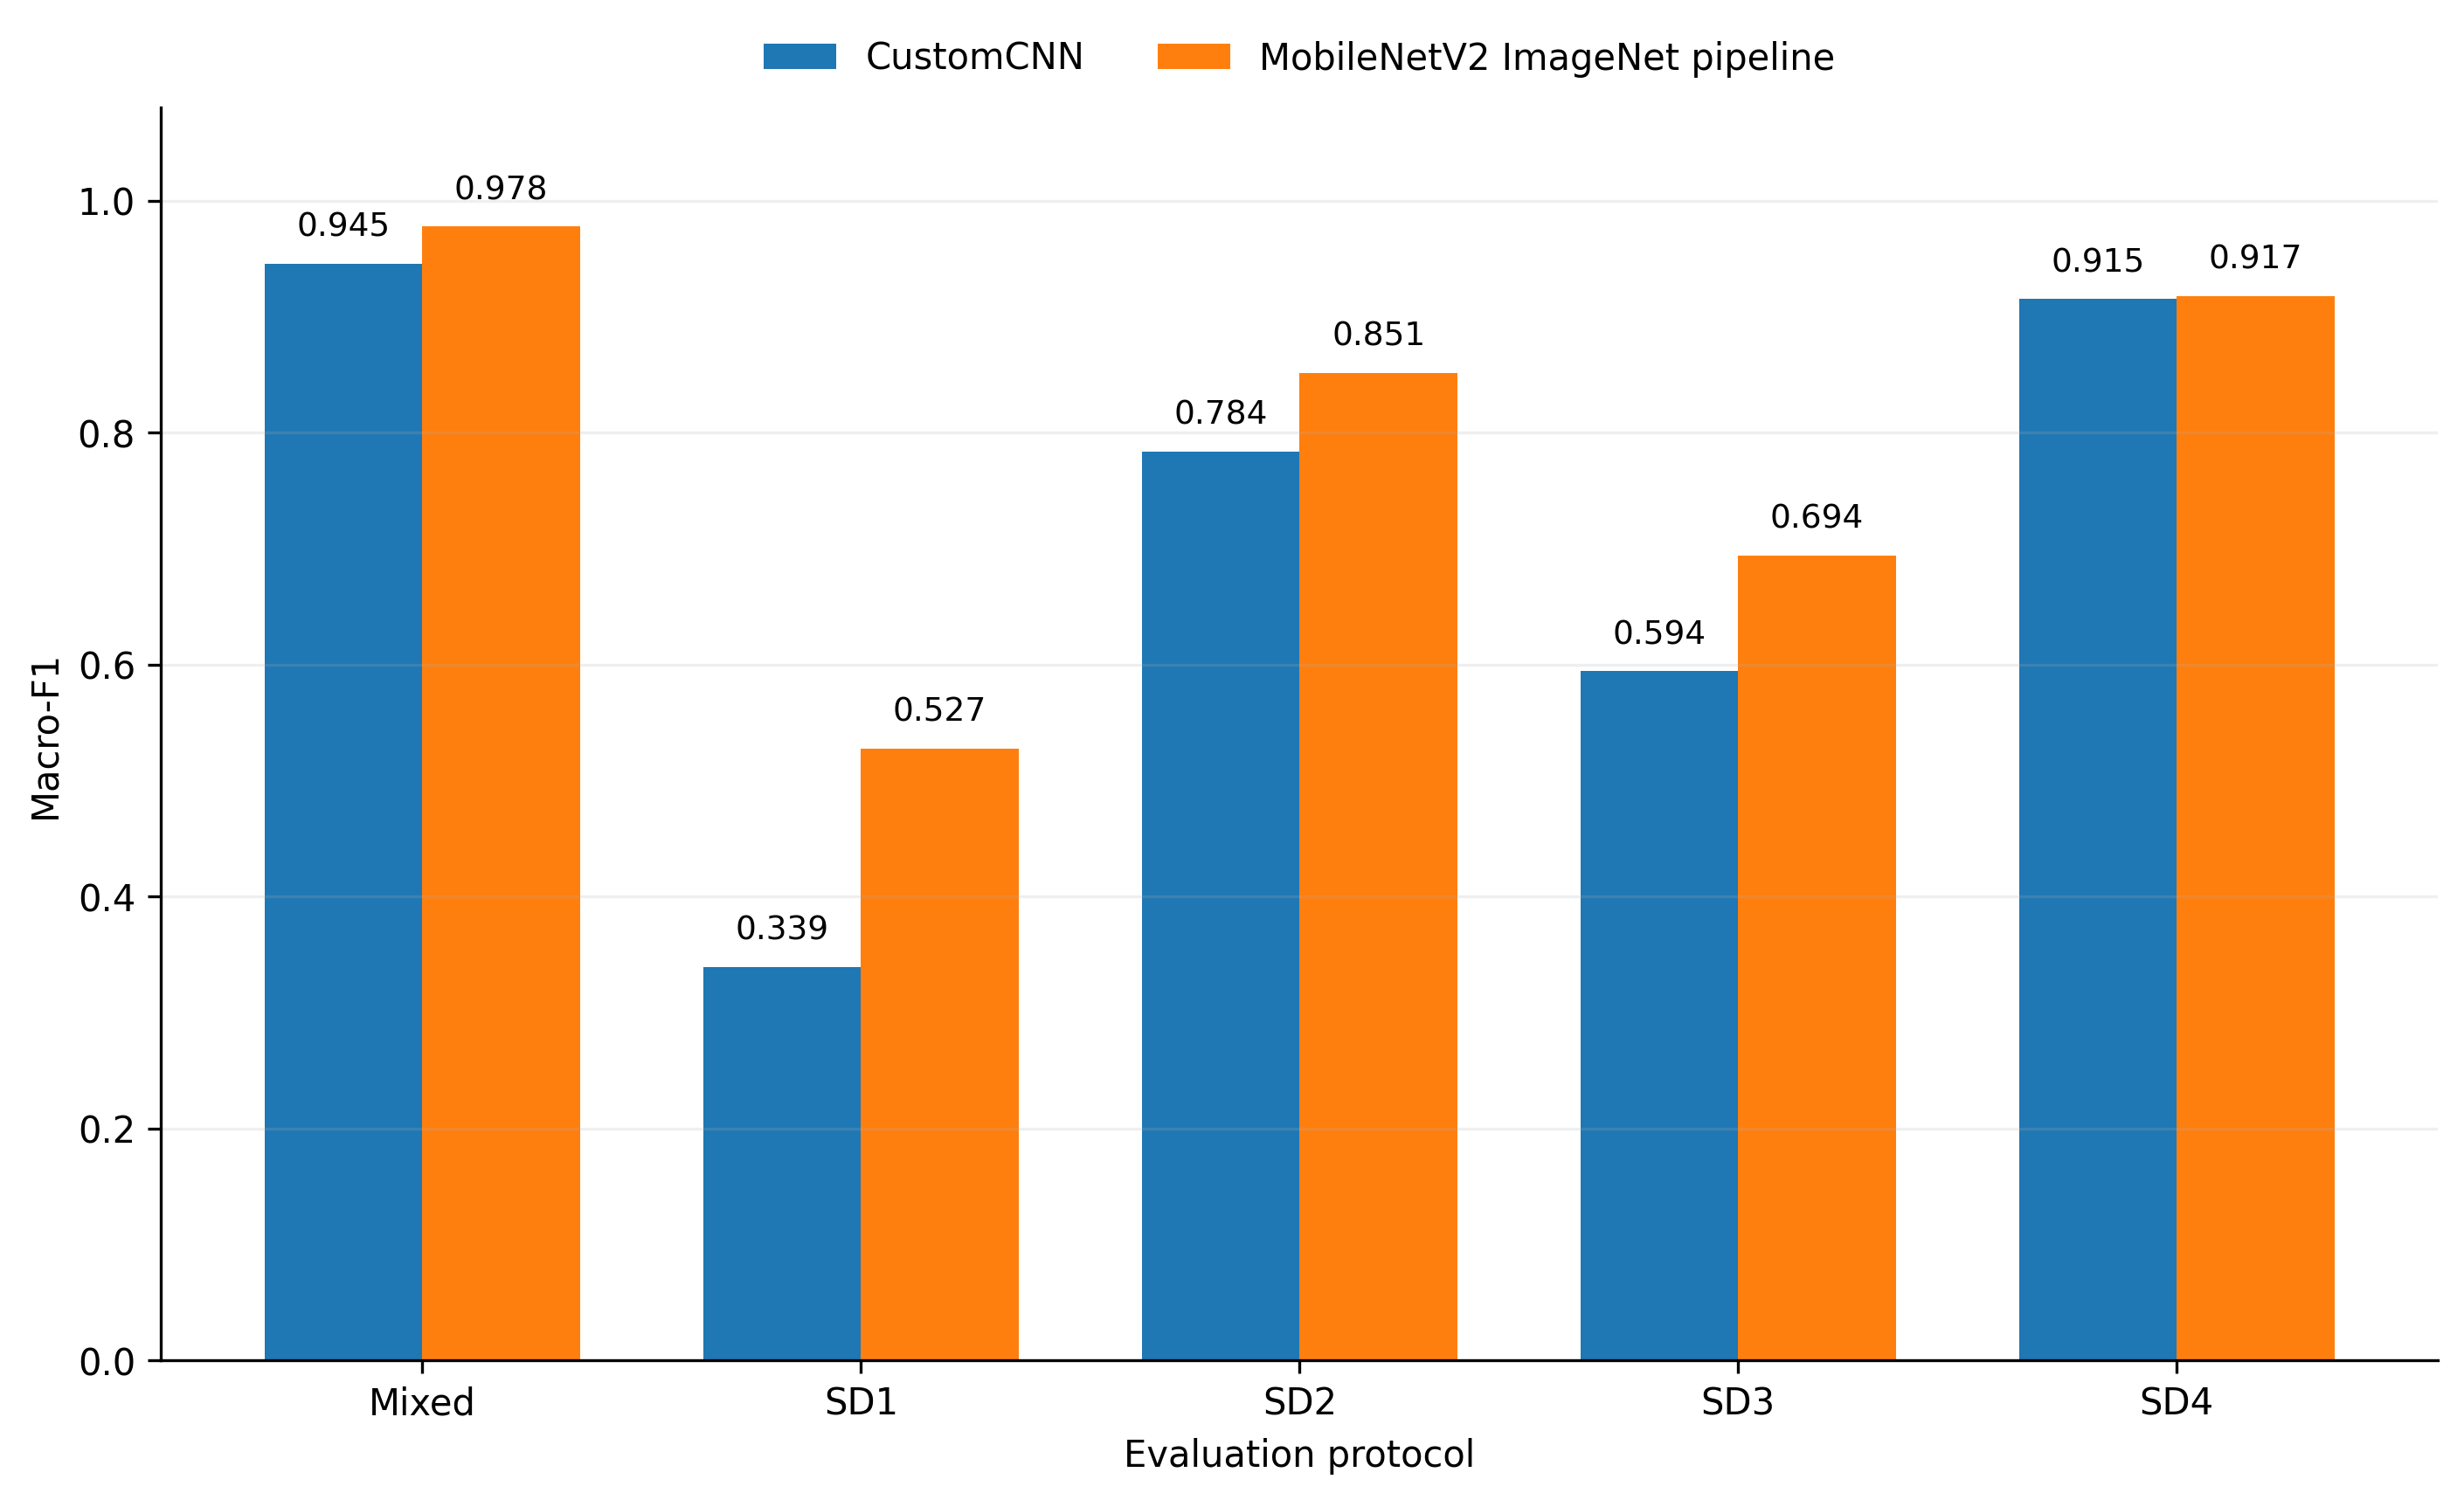
\includegraphics[width=0.84\textwidth]
{Fig_Mixed_vs_Source_Disjoint_MacroF1.png}
\caption{
Macro-F1 under mixed and source-disjoint evaluation.
Both pipelines achieve strong mixed-split performance but deteriorate
on unseen sources, particularly SD1. MobileNetV2 decreases from
0.9775 under mixed evaluation to 0.5274 on SD1, corresponding to a
45.0-percentage-point drop.
}
\label{fig:mixed_source}
\end{figure*}

Across SD1--SD4, CustomCNN achieves mean Macro-F1 0.6579 and
MobileNetV2 achieves 0.7476, an observed difference of 8.97 percentage
points. This should not be attributed solely to ImageNet pretraining
because architecture and training strategy also differ.

The substantial variation across the source-disjoint folds further
shows that apparent robustness depends strongly on which image sources
are withheld.

% ============================================================
% B. MULTI-SEED DG
% ============================================================

\subsection{Three-Seed Domain-Generalization Evaluation}


\begin{table}[t]
\centering
\caption{SD1 Three-Seed Replication}
\label{tab:sd1_multiseed}
\begin{tabular}{lcc}
\hline
Method & Seeds & Macro-F1 \\
\hline
ERM & 42, 123, 2026 & 0.4988$\pm$0.0259 \\
DG-AUG-V2 & 42, 123, 2026 & 0.4831$\pm$0.0443 \\
RSC & 42, 123, 2026 & 0.4883$\pm$0.0329 \\
\hline
\end{tabular}
\end{table}


ERM obtains $0.4988\pm0.0259$, DG-AUG-V2 obtains
$0.4831\pm0.0443$, and RSC obtains $0.4883\pm0.0329$.

Neither intervention consistently improves upon ERM. DG-AUG-V2 has a
lower mean and higher variability, whereas RSC is strongly
seed-sensitive. RSC improves over ERM for seed 2026 but performs worse
for seeds 42 and 123.

% ============================================================
% C. EXTERNAL FLOODNET
% ============================================================

\subsection{External FloodNet UAV Validation}


\begin{table*}[t]
\centering
\caption{Three-Seed Mean External FloodNet UAV Performance.
Supported Macro-F1 is computed over Flooded and Neither;
Desert predictions remain errors.}
\label{tab:floodnet_external}
\footnotesize
\setlength{\tabcolsep}{3.5pt}
\begin{tabular}{lccccccc}
\hline
Method & Acc. & Supp. F1 & AUROC & AUPRC &
Flood R. & Neither R. & False-Flood \\
\hline
ERM & 0.3886 & 0.3753$\pm$0.0468 & 0.7820 & 0.6305 & 0.9542 & 0.3055 & 0.6907 \\
DG-AUG-V2 & 0.3886 & 0.3729$\pm$0.0824 & 0.7730 & 0.6392 & 0.9477 & 0.3064 & 0.6907 \\
RSC & 0.3735 & 0.3619$\pm$0.0764 & 0.7848 & 0.6300 & 0.9804 & 0.2843 & 0.7109 \\
\hline
\end{tabular}
\end{table*}


ERM obtains supported-class Macro-F1
$0.3753\pm0.0468$. DG-AUG-V2 and RSC obtain
$0.3729\pm0.0824$ and $0.3619\pm0.0764$, respectively.

For ERM, mean Flooded recall is 0.9542 and mean Neither recall is
0.3055.

Among 347 external true-Neither scenes:

\begin{itemize}
    \item 178 (51.3\%) are predicted Flooded by all nine models,
    \item 56 (16.1\%) are predicted Neither by all nine models,
    \item 113 (32.6\%) show disagreement.
\end{itemize}

The agreement across methods and seeds indicates that this external
error is systematic rather than specific to a single model run.

% ============================================================
% COMBINE FORMER FIGURES 2 + 3
% ============================================================

\begin{figure*}[!t]
\centering

\begin{minipage}[t]{0.485\textwidth}
    \centering
    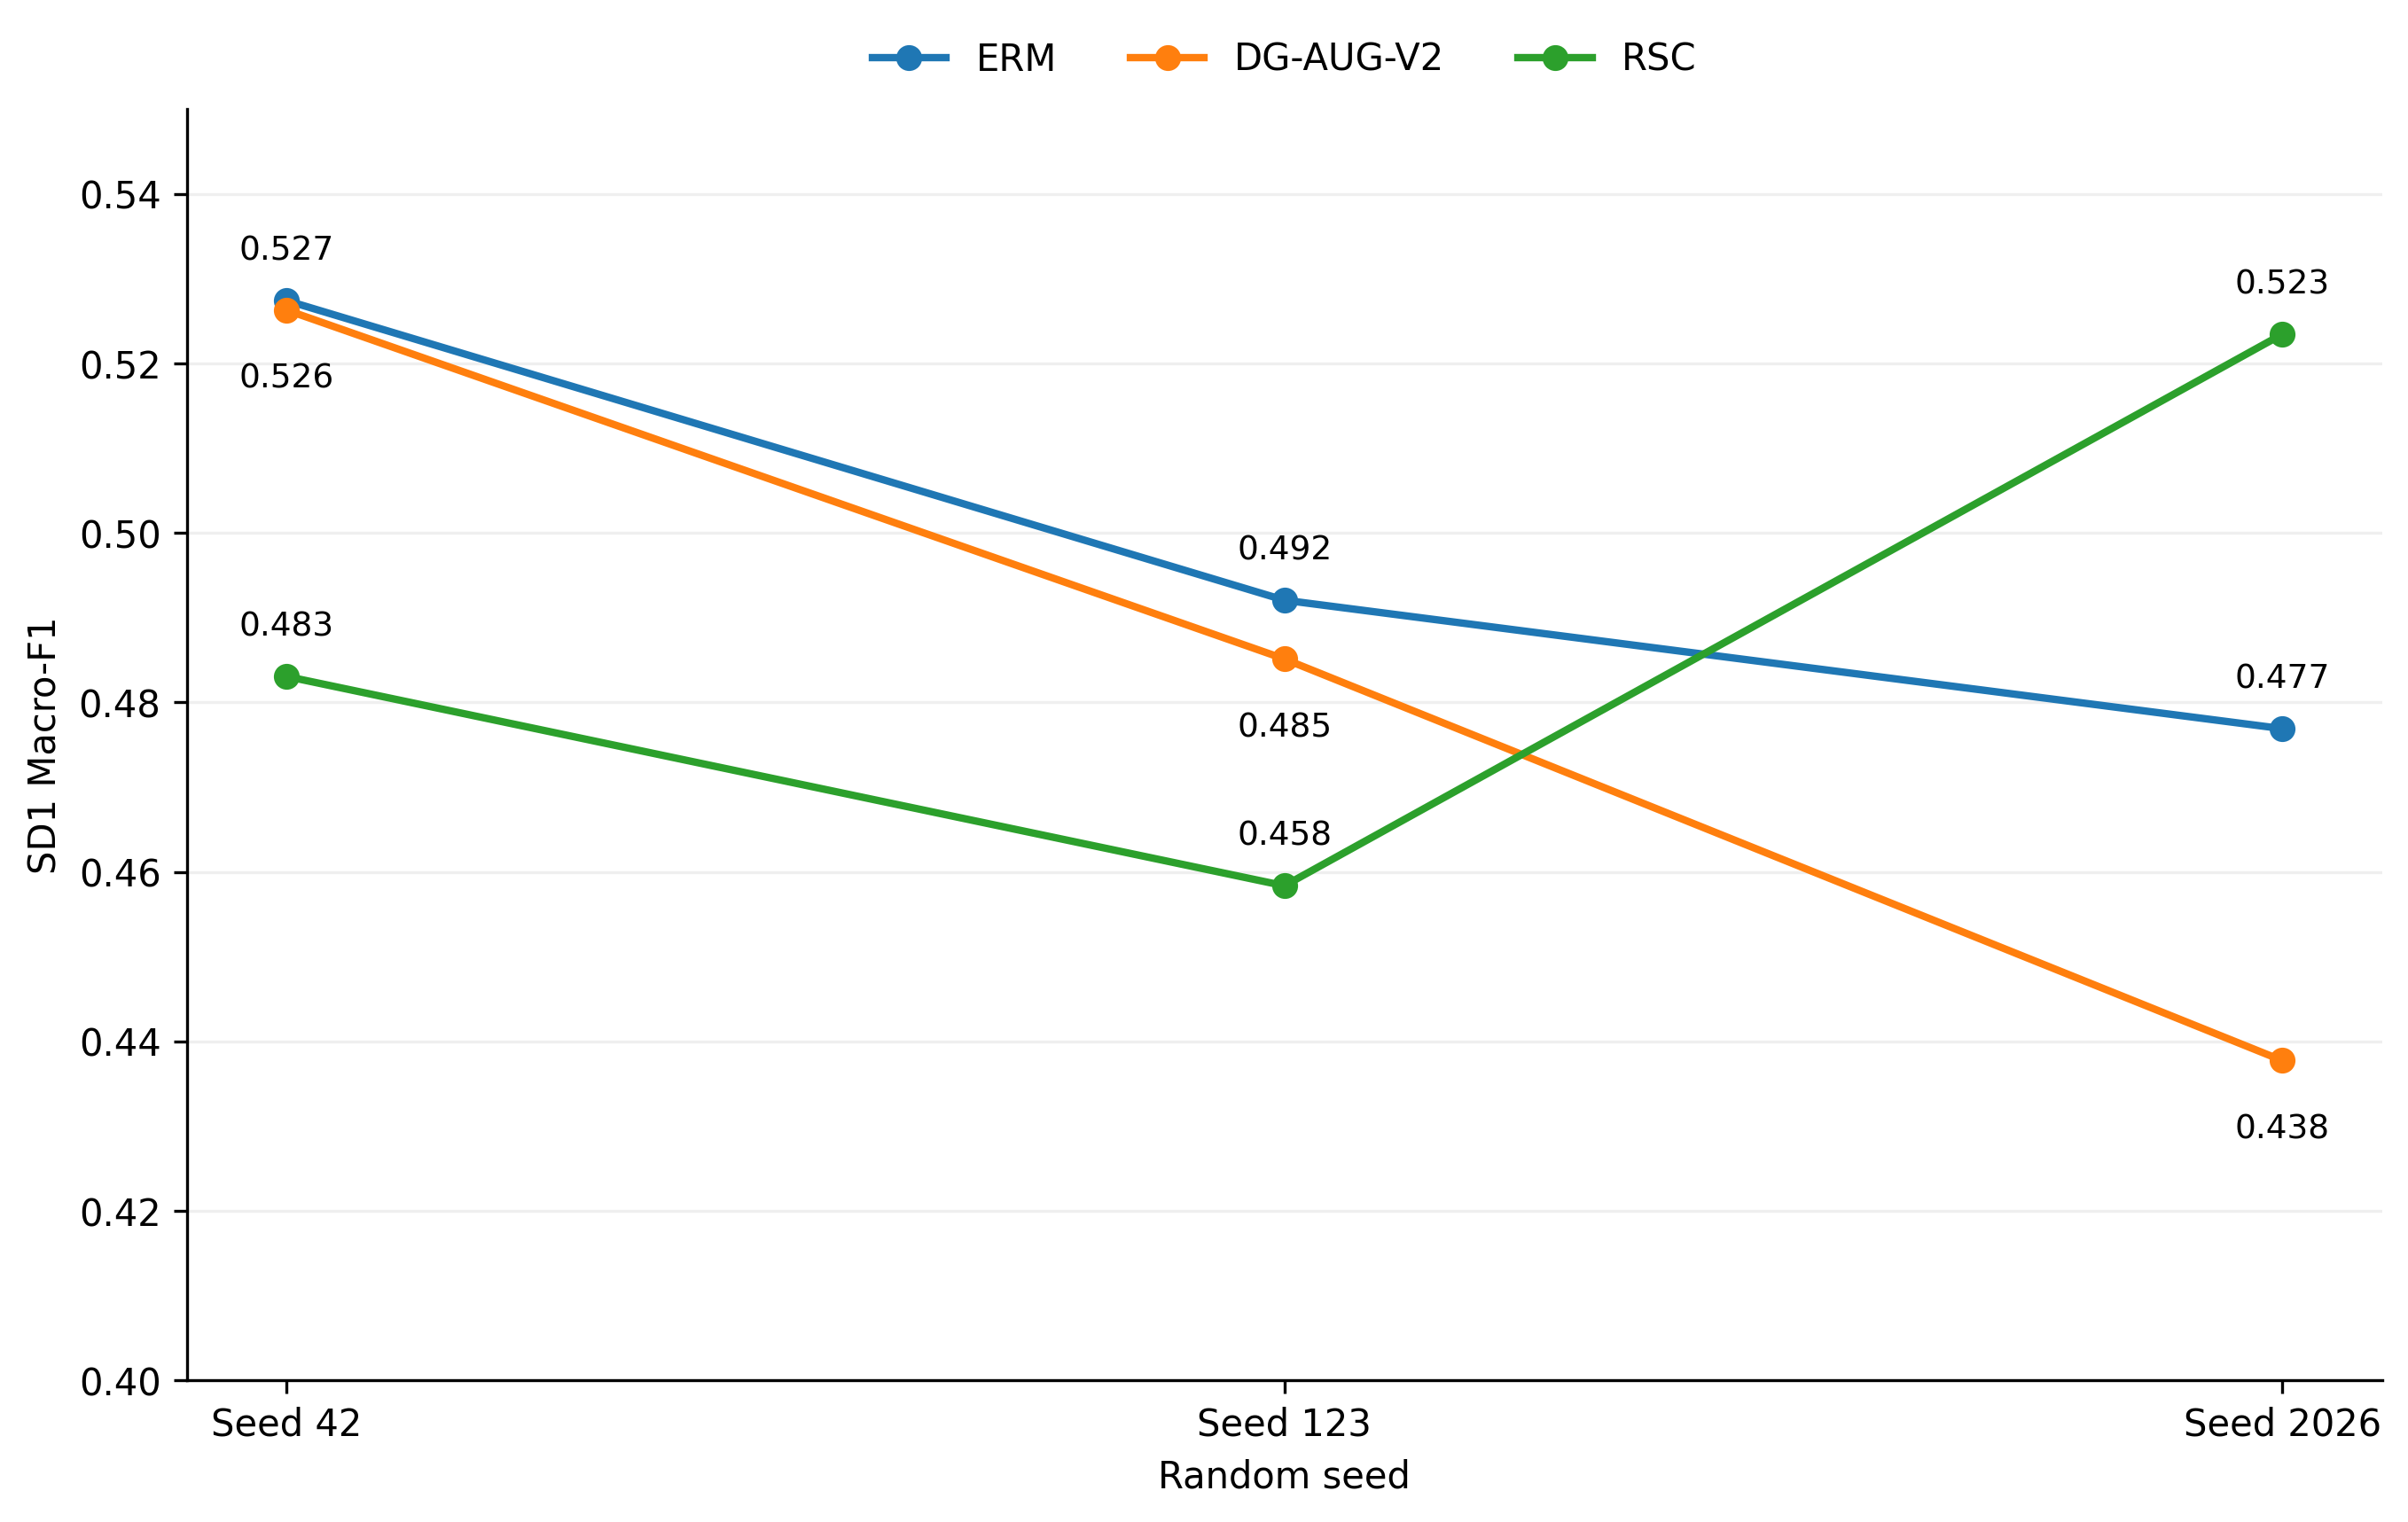
\includegraphics[width=\linewidth]
    {Fig_SD1_ThreeSeed_Method_Comparison.png}

    \vspace{-1mm}
    \textbf{(a)}
\end{minipage}
\hfill
\begin{minipage}[t]{0.485\textwidth}
    \centering
    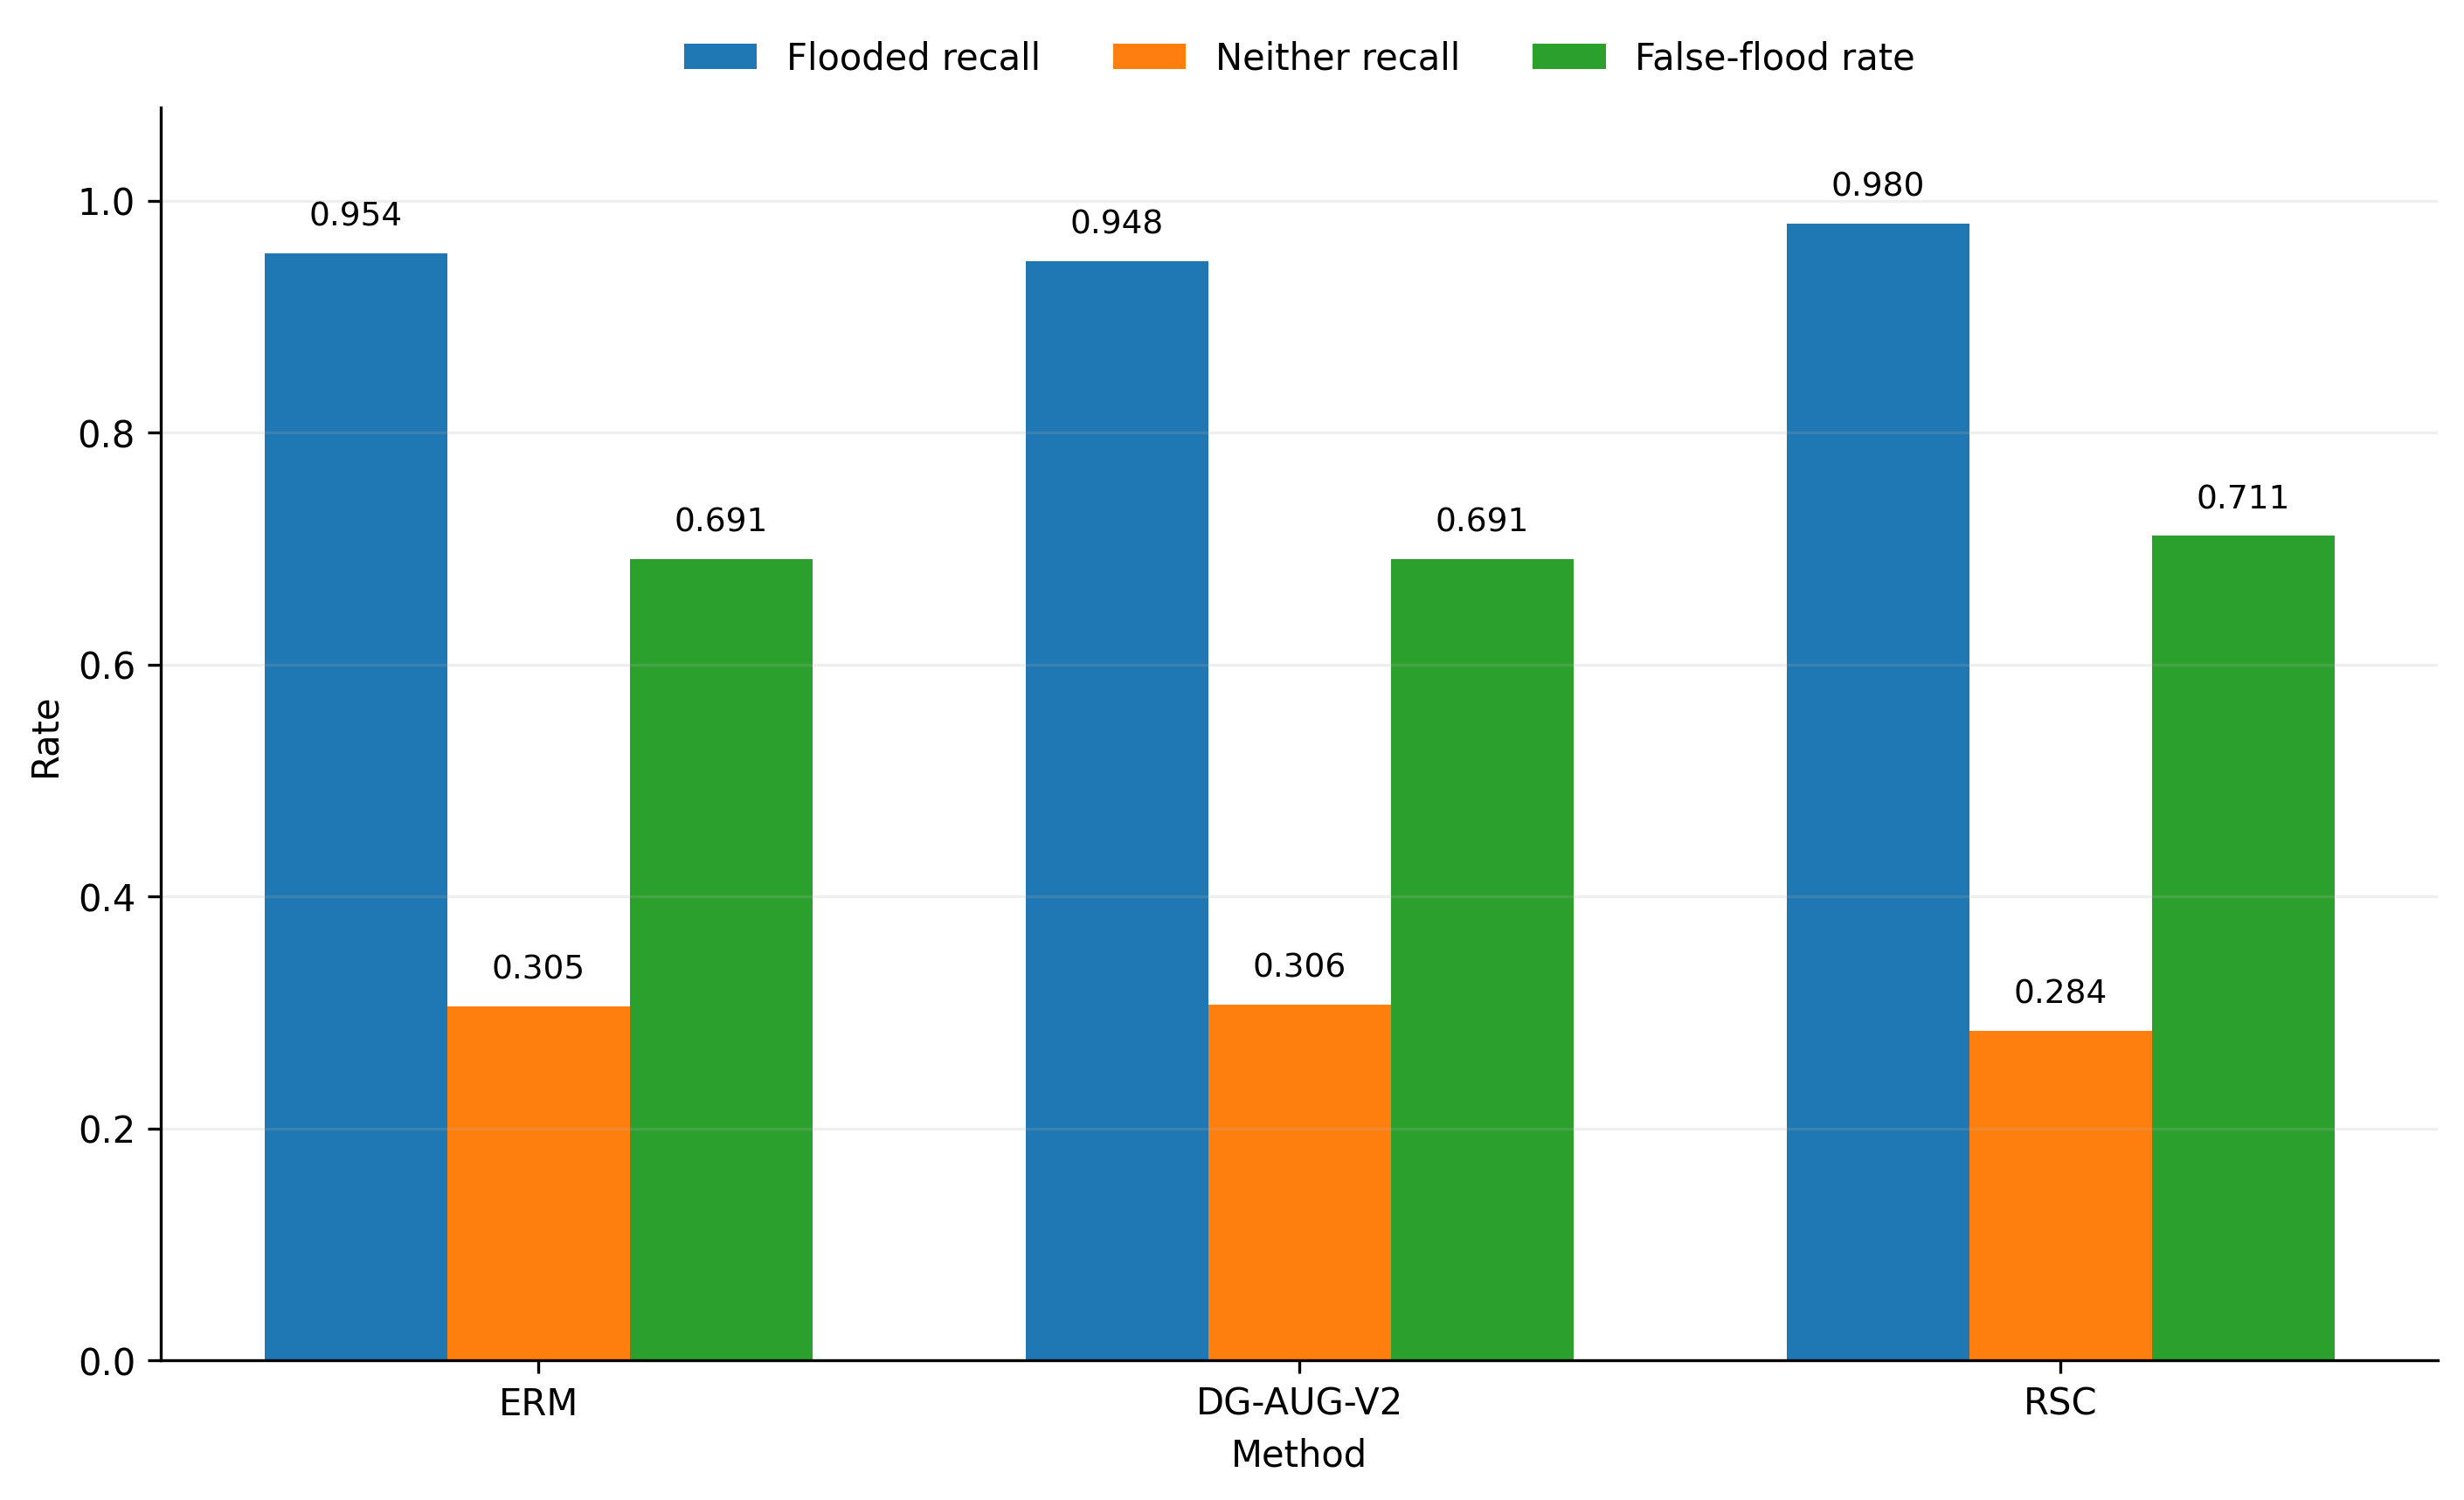
\includegraphics[width=\linewidth]
    {Fig_FloodNet_External_Asymmetric_Failure.png}

    \vspace{-1mm}
    \textbf{(b)}
\end{minipage}

\caption{
Robustness evaluation beyond the mixed split.
(a) SD1 Macro-F1 across seeds 42, 123, and 2026. RSC underperforms
ERM on two seeds but exceeds it on seed 2026, illustrating the danger
of drawing conclusions from a single favorable run.
(b) External FloodNet UAV evaluation. All three methods retain high
Flooded recall but exhibit low Neither recall and high false-flood
rates.
}
\label{fig:robustness_pair}
\end{figure*}

% ============================================================
% D. GRAD-CAM
% ============================================================

\subsection{Grad-CAM Analysis}

\begin{figure*}[!t]
\centering
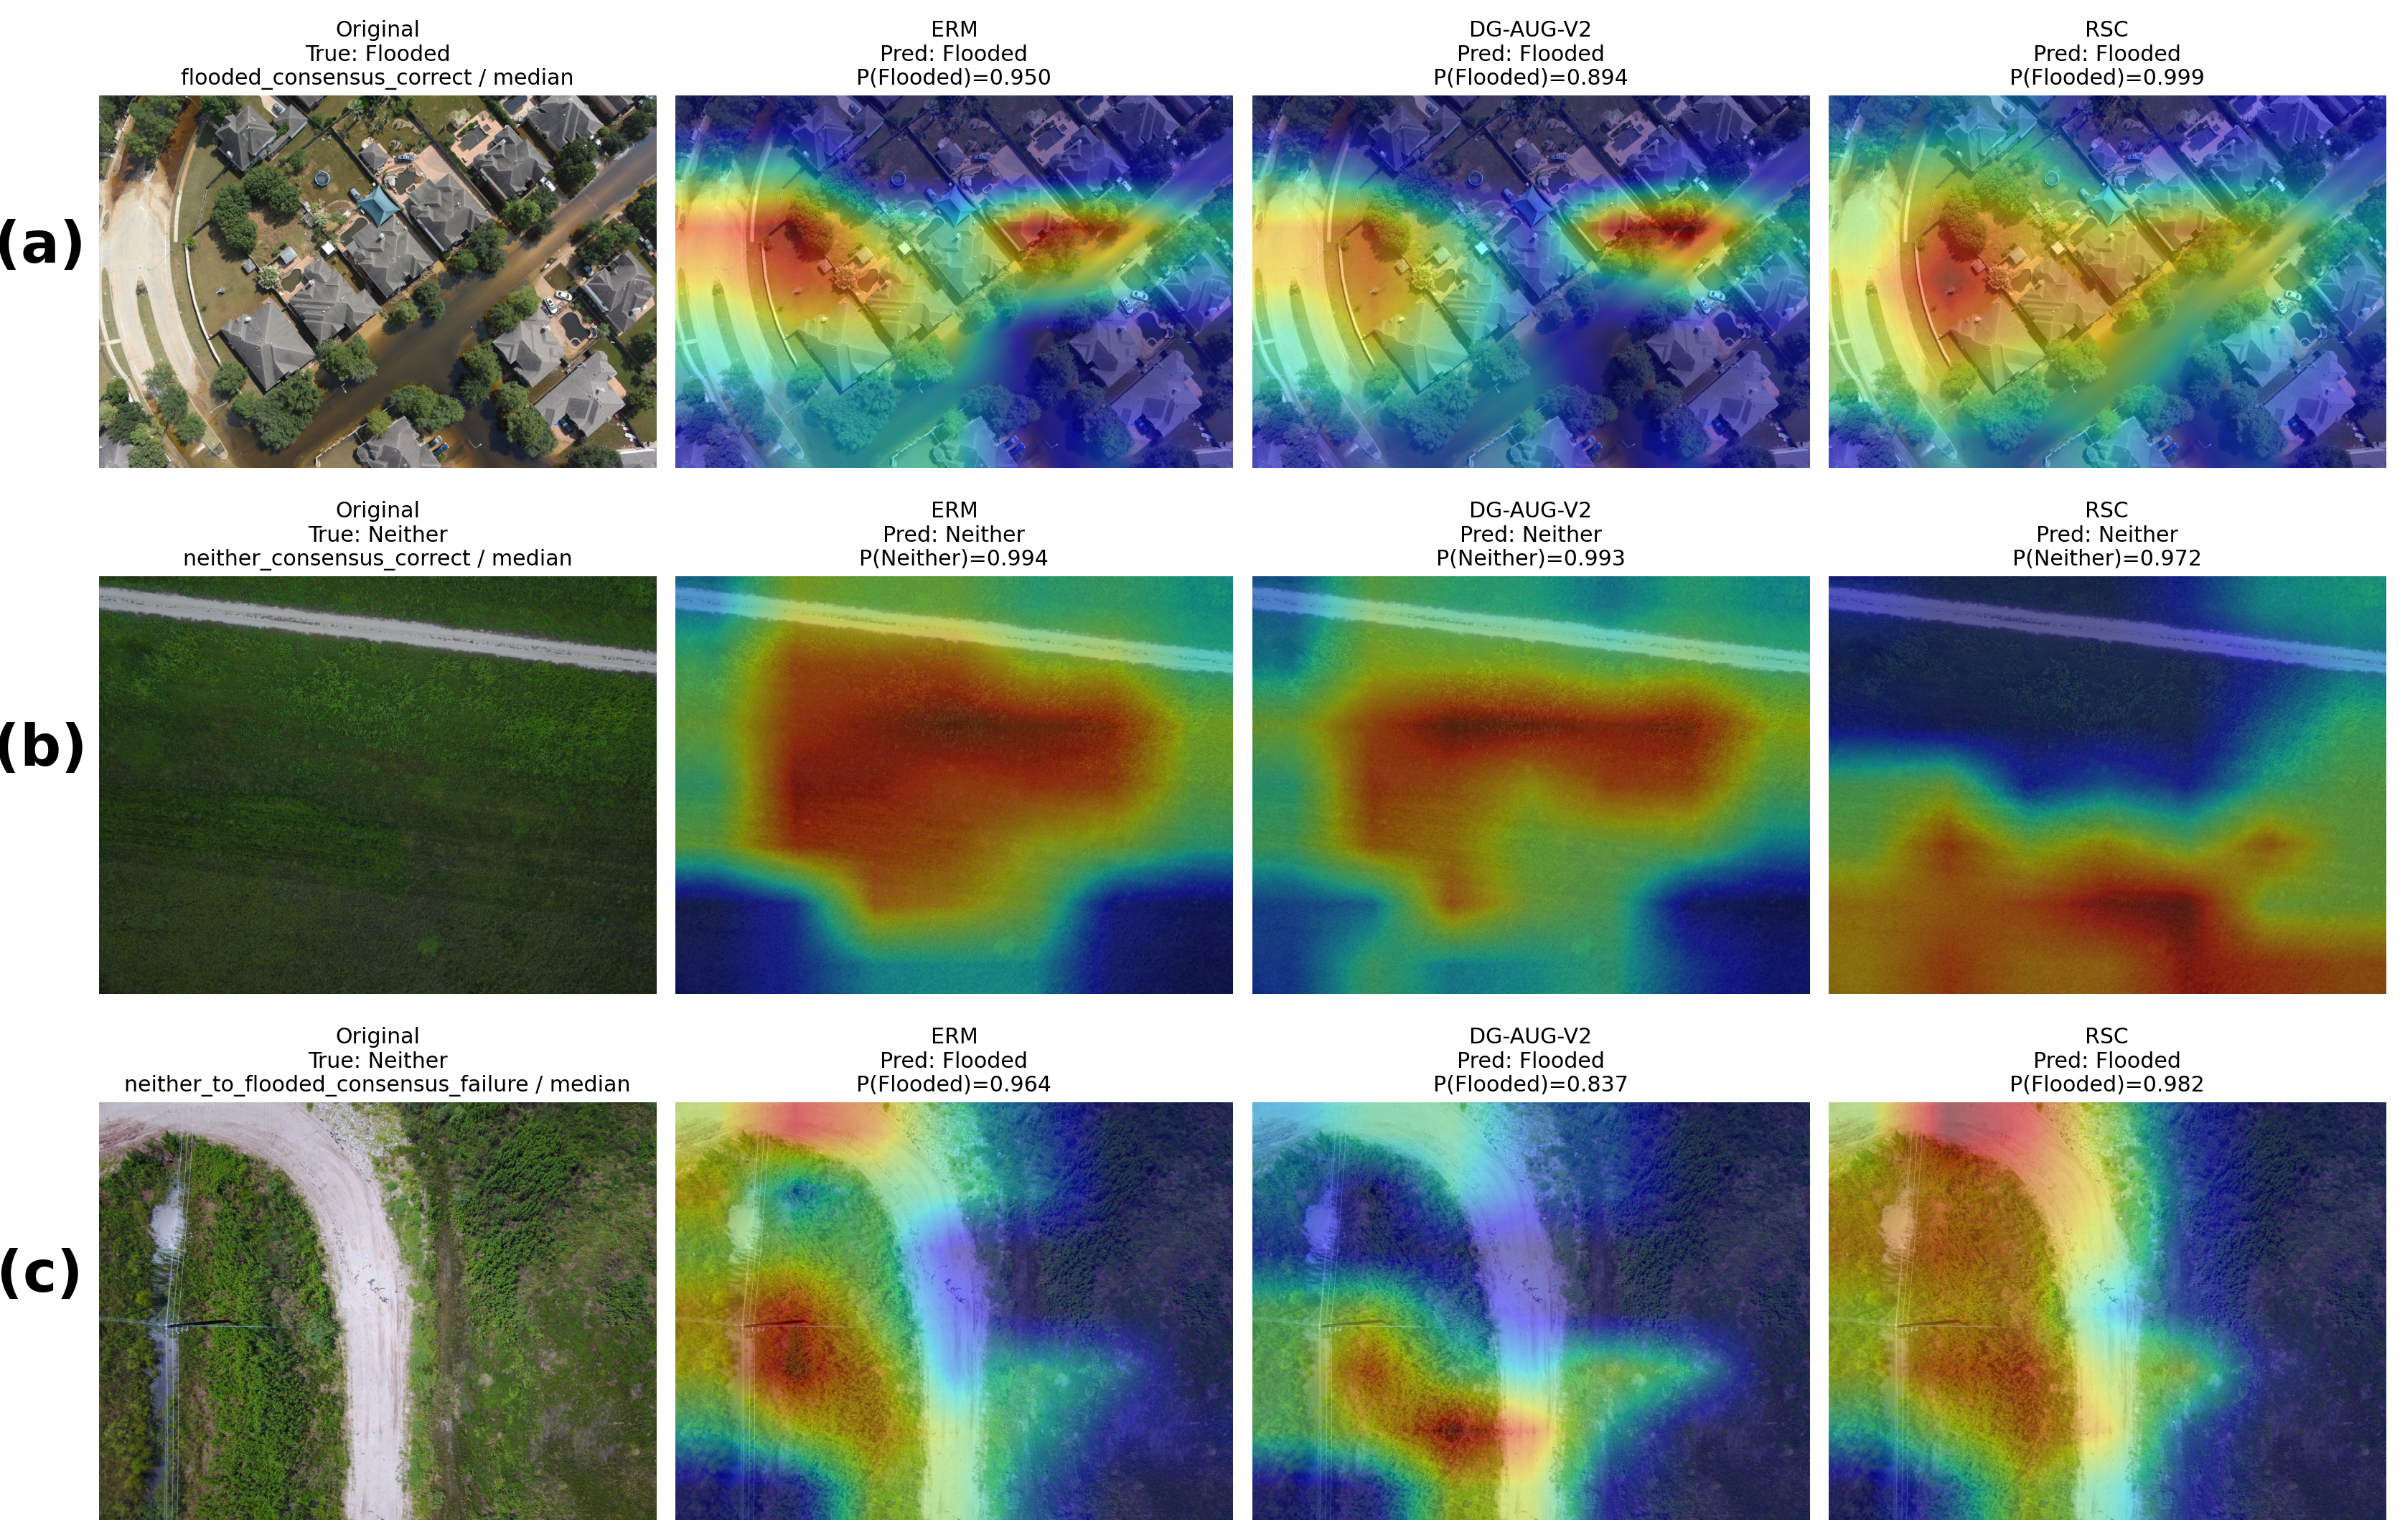
\includegraphics[width=0.92\textwidth]
{Fig_GradCAM_Representative_Median_Cases.png}
\caption{
Representative Grad-CAM visualizations from the frozen
median-confidence cohort.
(a) Consensus-correct Flooded scene,
(b) consensus-correct Neither scene, and
(c) consensus Neither-to-Flooded failure.
Columns show the original image and Grad-CAM maps from ERM,
DG-AUG-V2, and RSC.
}
\label{fig:gradcam}
\end{figure*}

Correct Neither scenes frequently emphasize homogeneous vegetation
and land texture. Several false-flood cases instead emphasize
water-like regions, roads, boundaries, and adjacent infrastructure.

ERM and DG-AUG-V2 often produce similar spatial activation patterns,
whereas RSC tends to produce broader or spatially shifted activation.

These maps are qualitative explanatory evidence and are not interpreted
as causal proof of the model's decision process.

% ============================================================
% E. SEGMENTATION SHORTCUT ANALYSIS
% ============================================================

\subsection{Segmentation-Based Failure Analysis}


\begin{table*}[t]
\centering
\caption{Post-Hoc Segmentation Composition of Consensus
False-Flood ($n=178$) and Consensus-Correct Neither ($n=56$)
Scenes. Reported $p$-values are Holm-adjusted across all ten
segmentation classes. Road-flooded and Building-flooded pixels
were absent from both consensus groups.}
\label{tab:segmentation_shortcut}
\footnotesize
\setlength{\tabcolsep}{4pt}
\begin{tabular}{lrrrrrr}
\hline
Class &
Fail Pres. (\%) &
Corr. Pres. (\%) &
Fail Area (\%) &
Corr. Area (\%) &
Fisher $p_{\mathrm{Holm}}$ &
MW $p_{\mathrm{Holm}}$ \\
\hline
Water & 51.7 & 5.4 & 13.44 & 0.53 & 2.42e-10 & 9.27e-09 \\
Road-non-flooded & 73.0 & 14.3 & 8.84 & 0.58 & 3.95e-14 & 3.85e-13 \\
Grass & 93.8 & 100.0 & 51.88 & 85.25 & 0.2823 & 2.02e-16 \\
Tree & 89.9 & 58.9 & 18.78 & 13.22 & 4.67e-06 & 5.18e-04 \\
\hline
\end{tabular}
\end{table*}


Water is present in 51.7\% of consensus false-flood scenes but only
5.4\% of consensus-correct Neither scenes. After Holm correction:

\[
p_{\mathrm{Holm}}=2.42\times10^{-10}.
\]

Non-flooded roads are present in 73.0\% of failures and 14.3\% of
correct scenes:

\[
p_{\mathrm{Holm}}=3.95\times10^{-14}.
\]

Grass presence itself is not significantly different after Holm
correction. However, mean Grass coverage is 51.88\% in failures and
85.25\% in correct scenes:

\[
p_{\mathrm{Holm}}=2.02\times10^{-16}.
\]

Road-flooded and Building-flooded pixels are absent from both
consensus groups.

% ============================================================
% COMBINE FORMER SEGMENTATION FIGURES 5 + 6
% ============================================================

\begin{figure*}[!t]
\centering

\begin{minipage}[t]{0.32\textwidth}
    \centering
    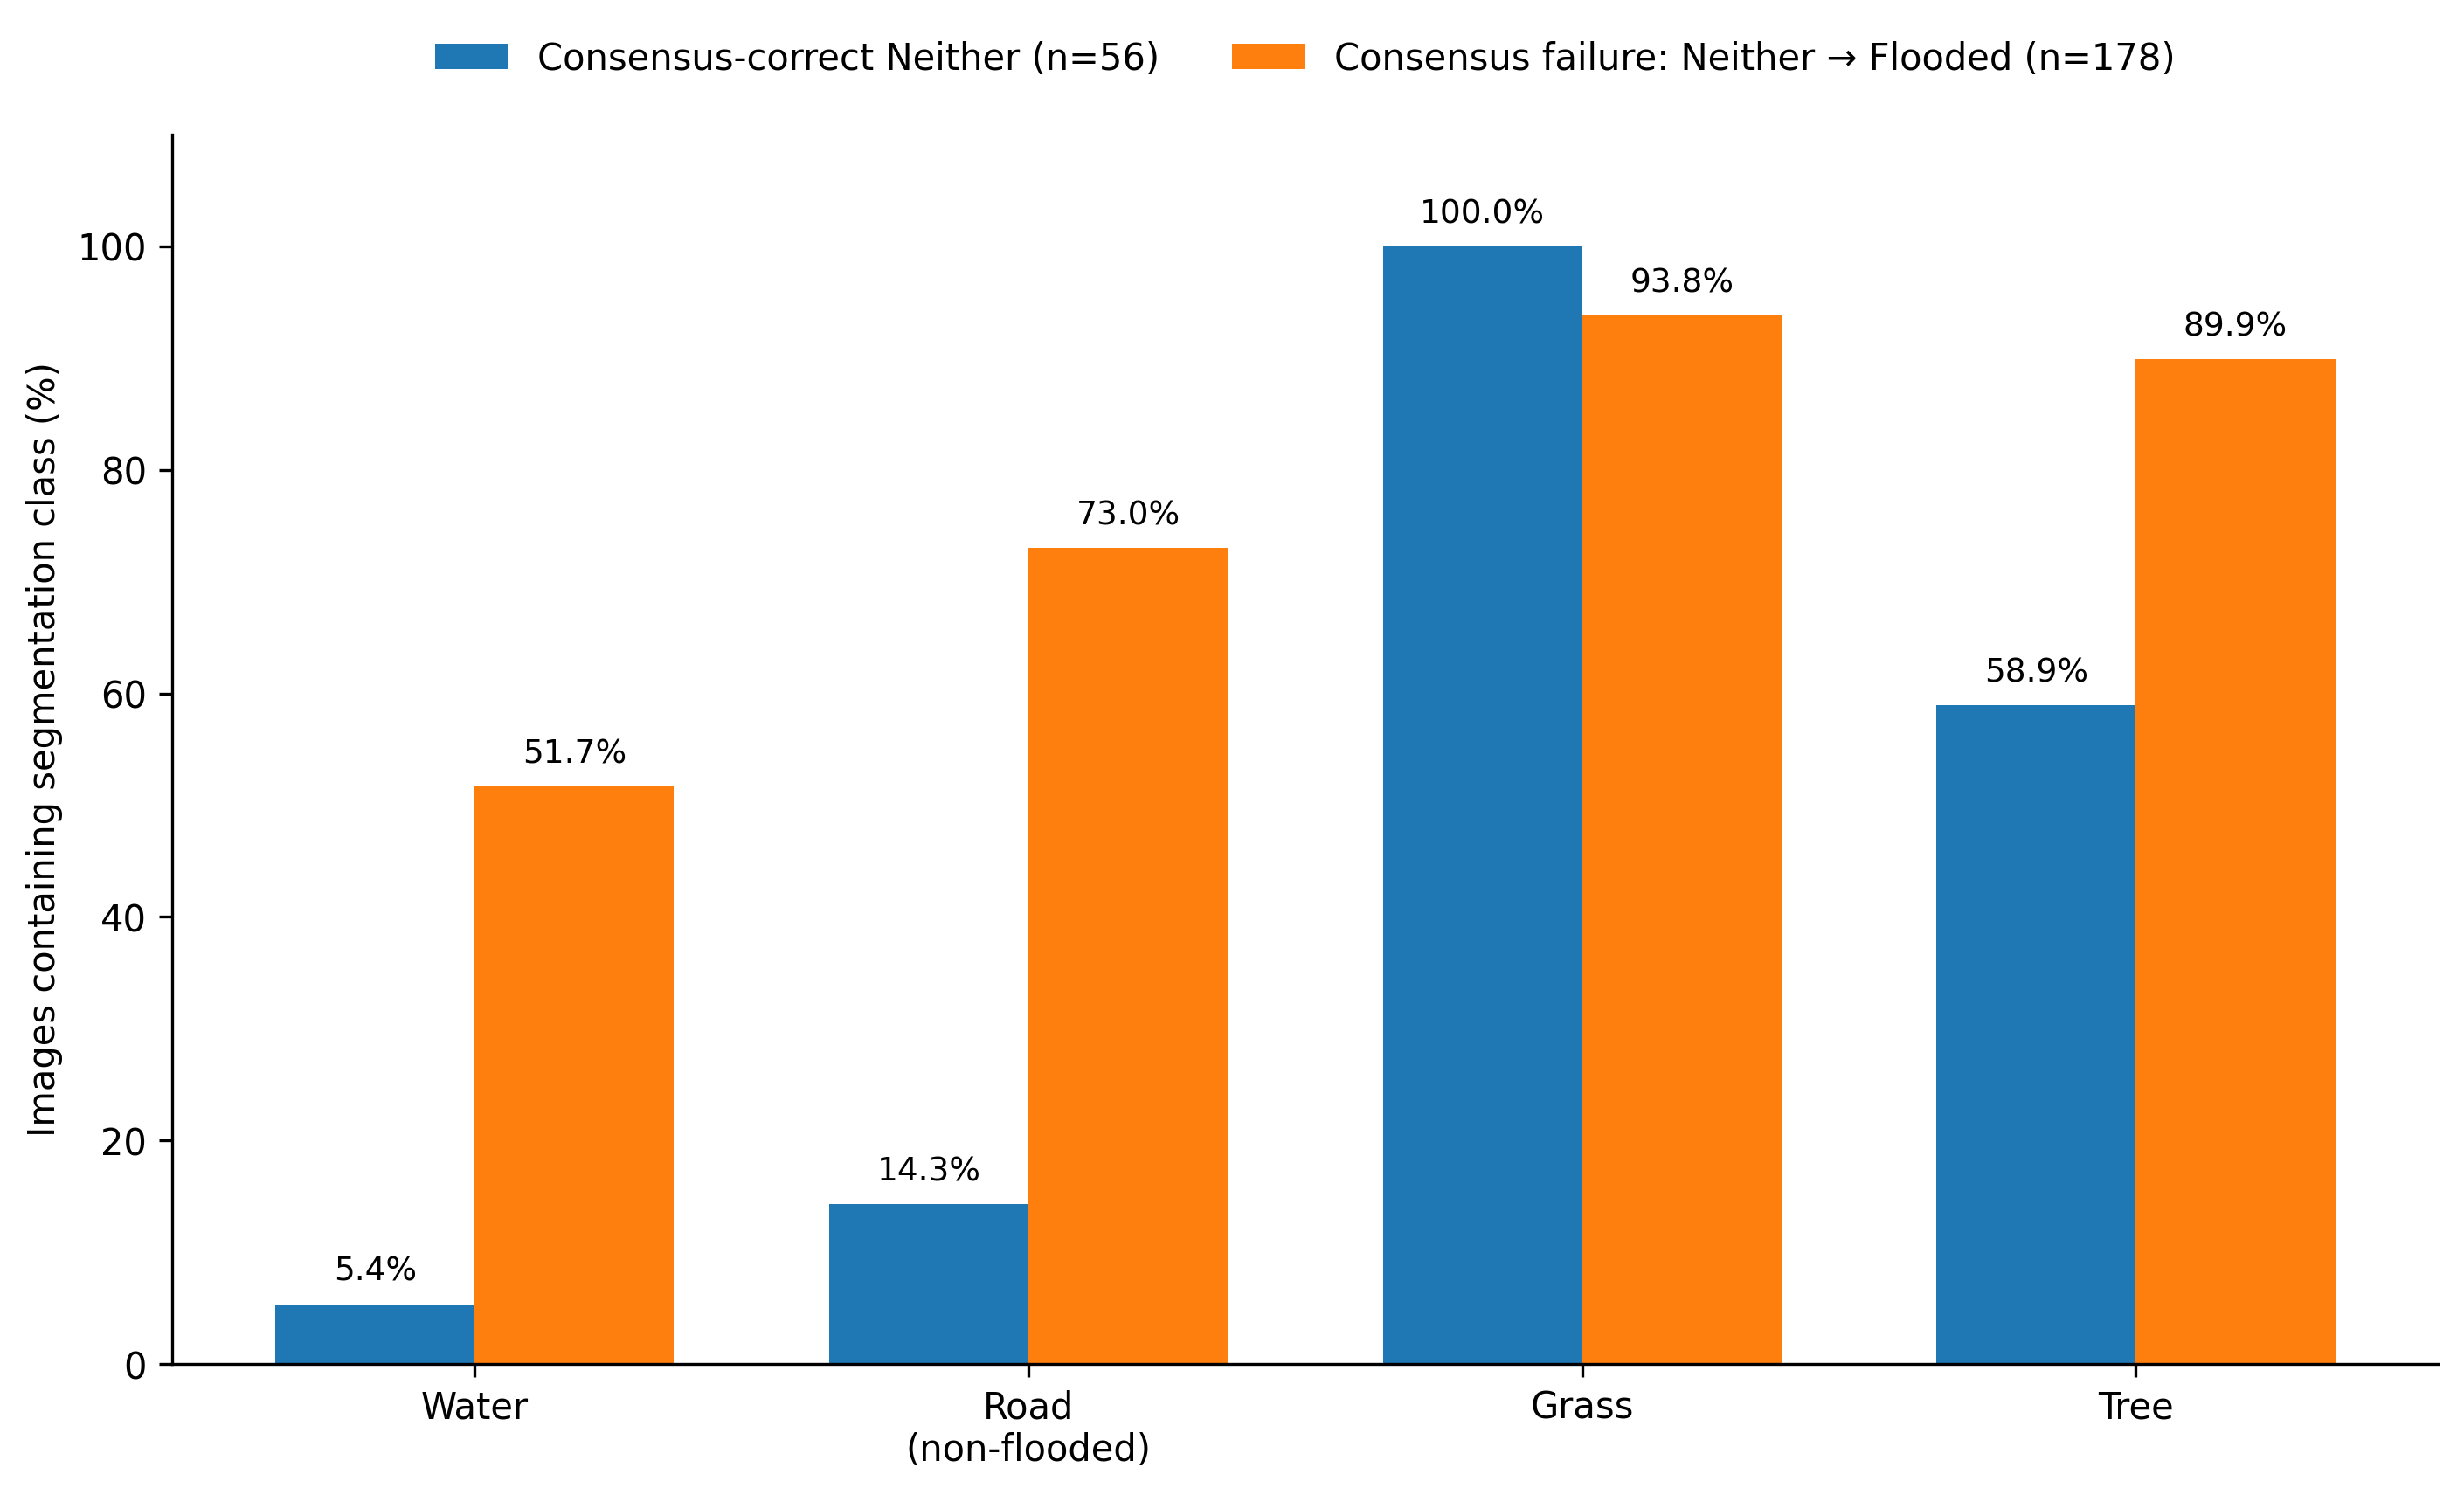
\includegraphics[width=\linewidth]
    {Fig_segmentation_class_presence_rates.png}

    \vspace{-1mm}
    \textbf{(a)}
\end{minipage}
\hfill
\begin{minipage}[t]{0.32\textwidth}
    \centering
    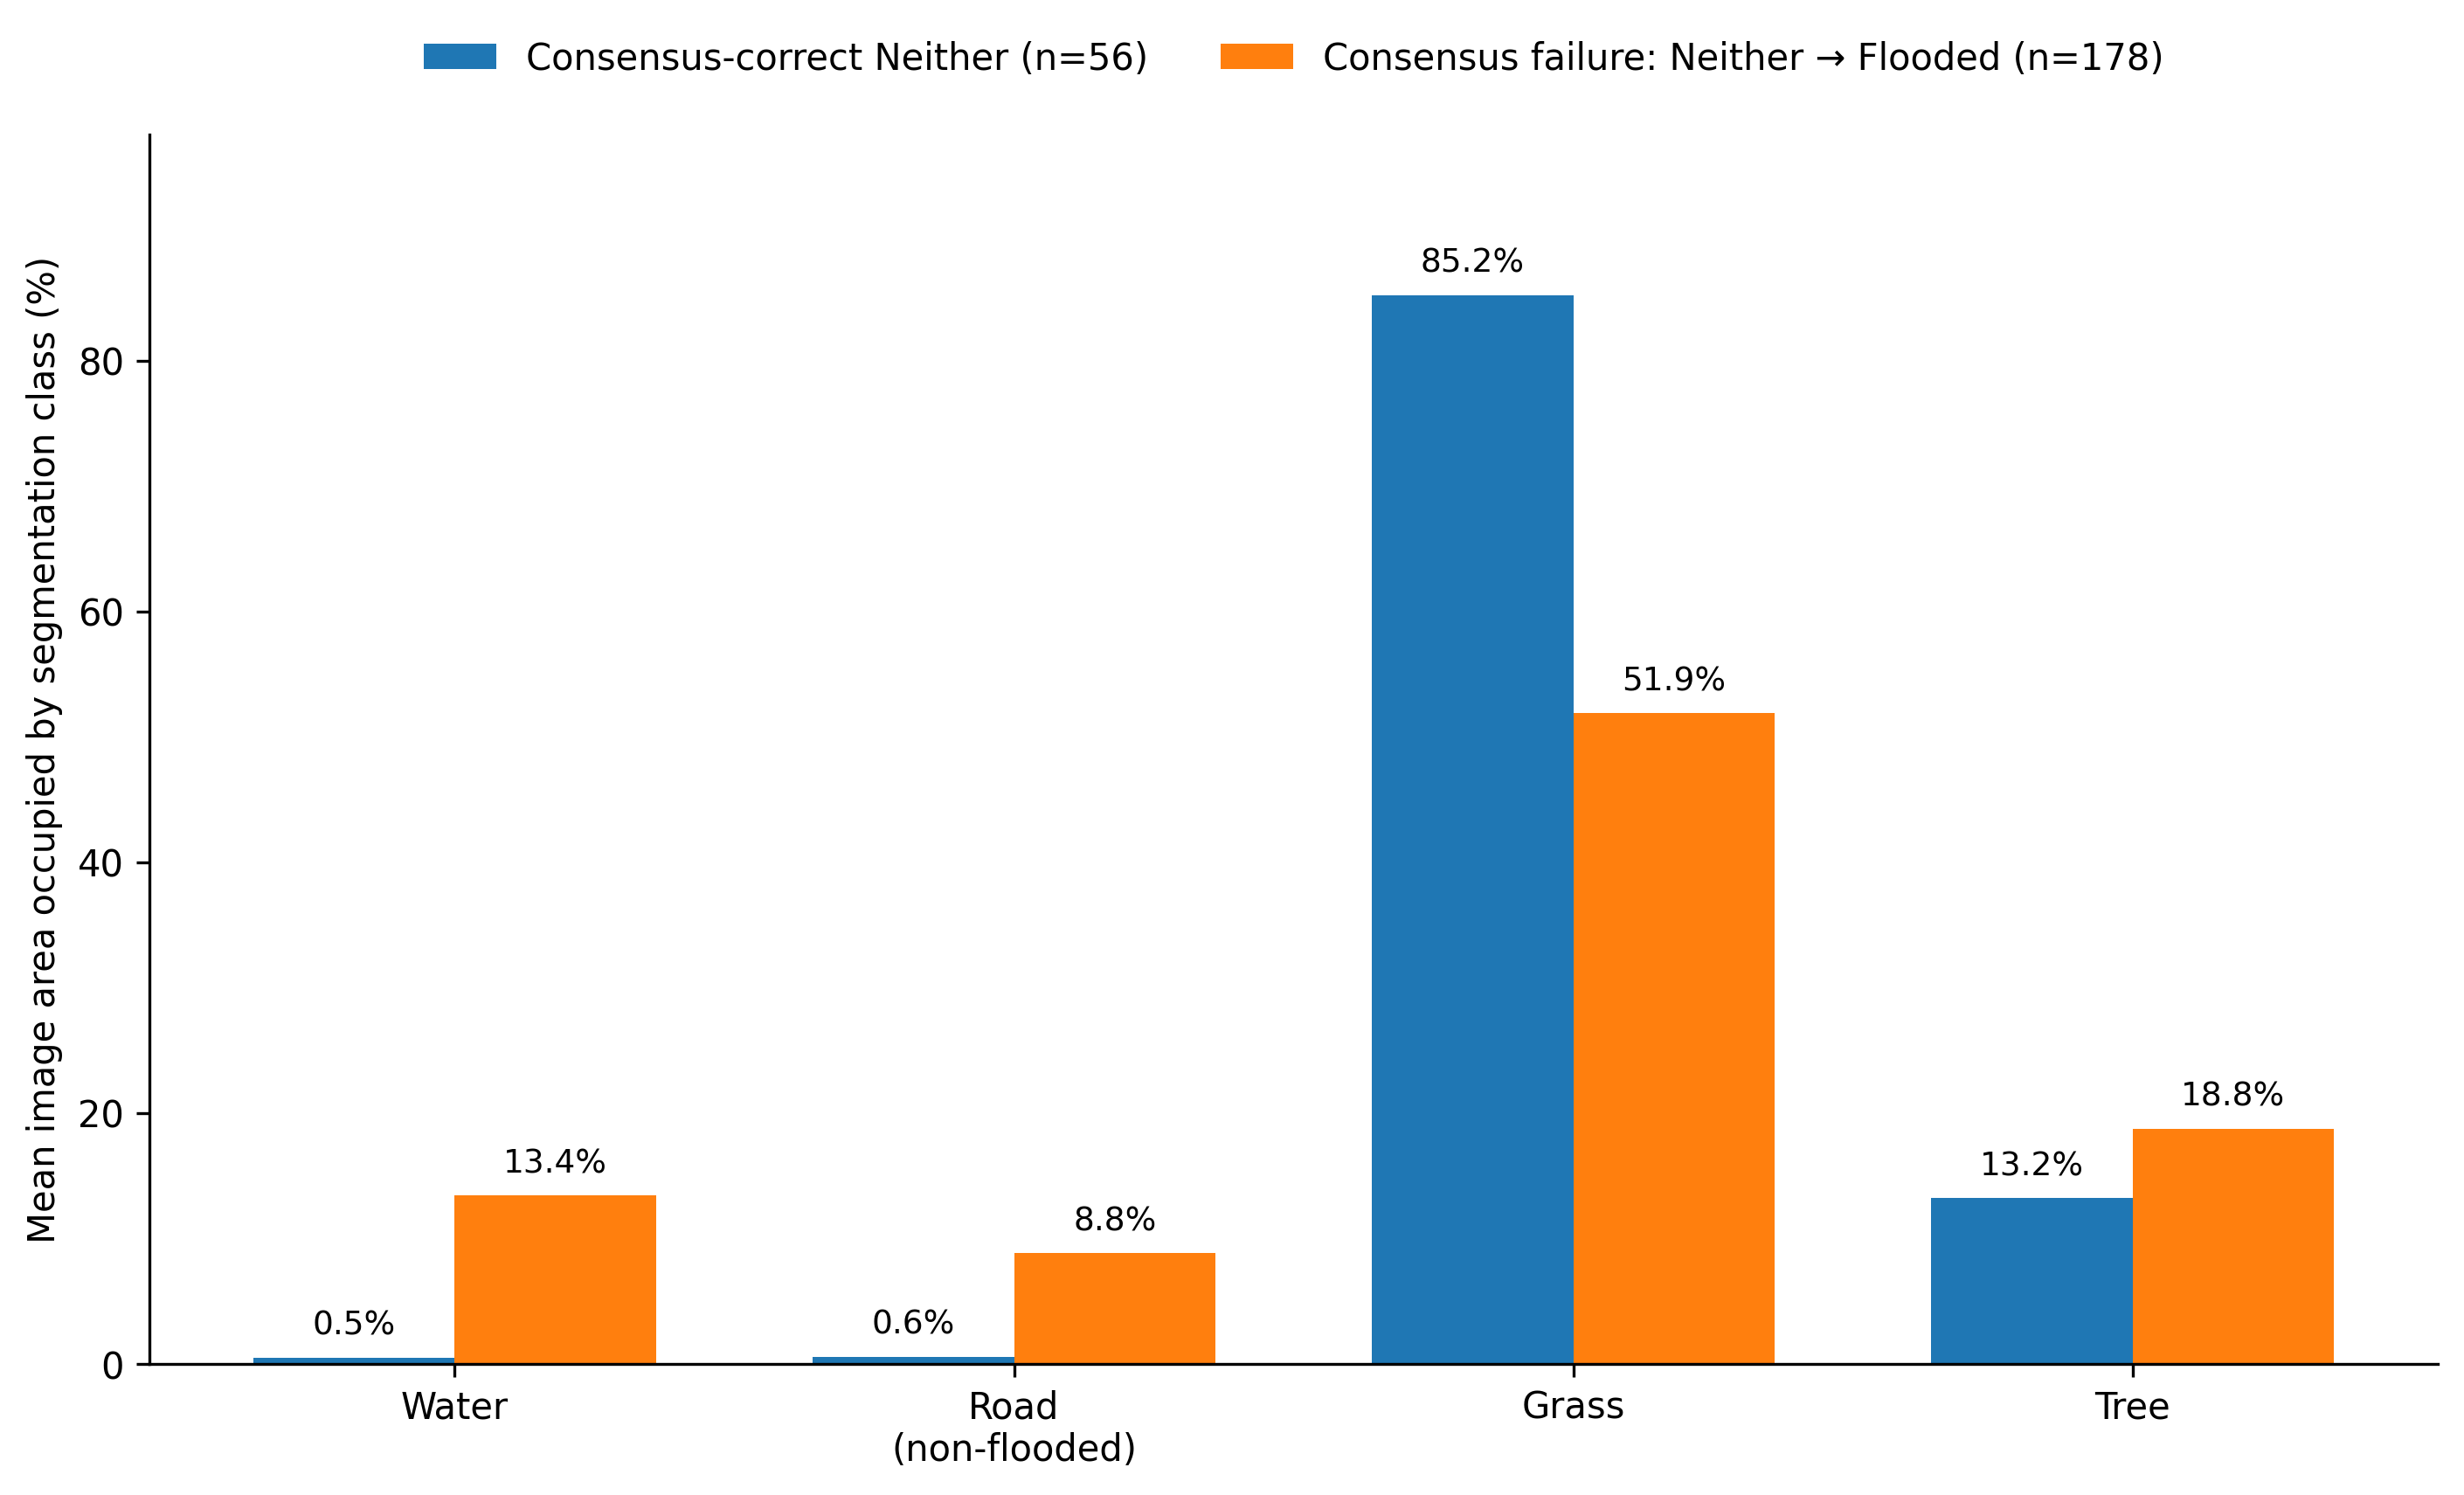
\includegraphics[width=\linewidth]
    {Fig_segmentation_mean_pixel_coverage.png}

    \vspace{-1mm}
    \textbf{(b)}
\end{minipage}
\hfill
\begin{minipage}[t]{0.32\textwidth}
    \centering
    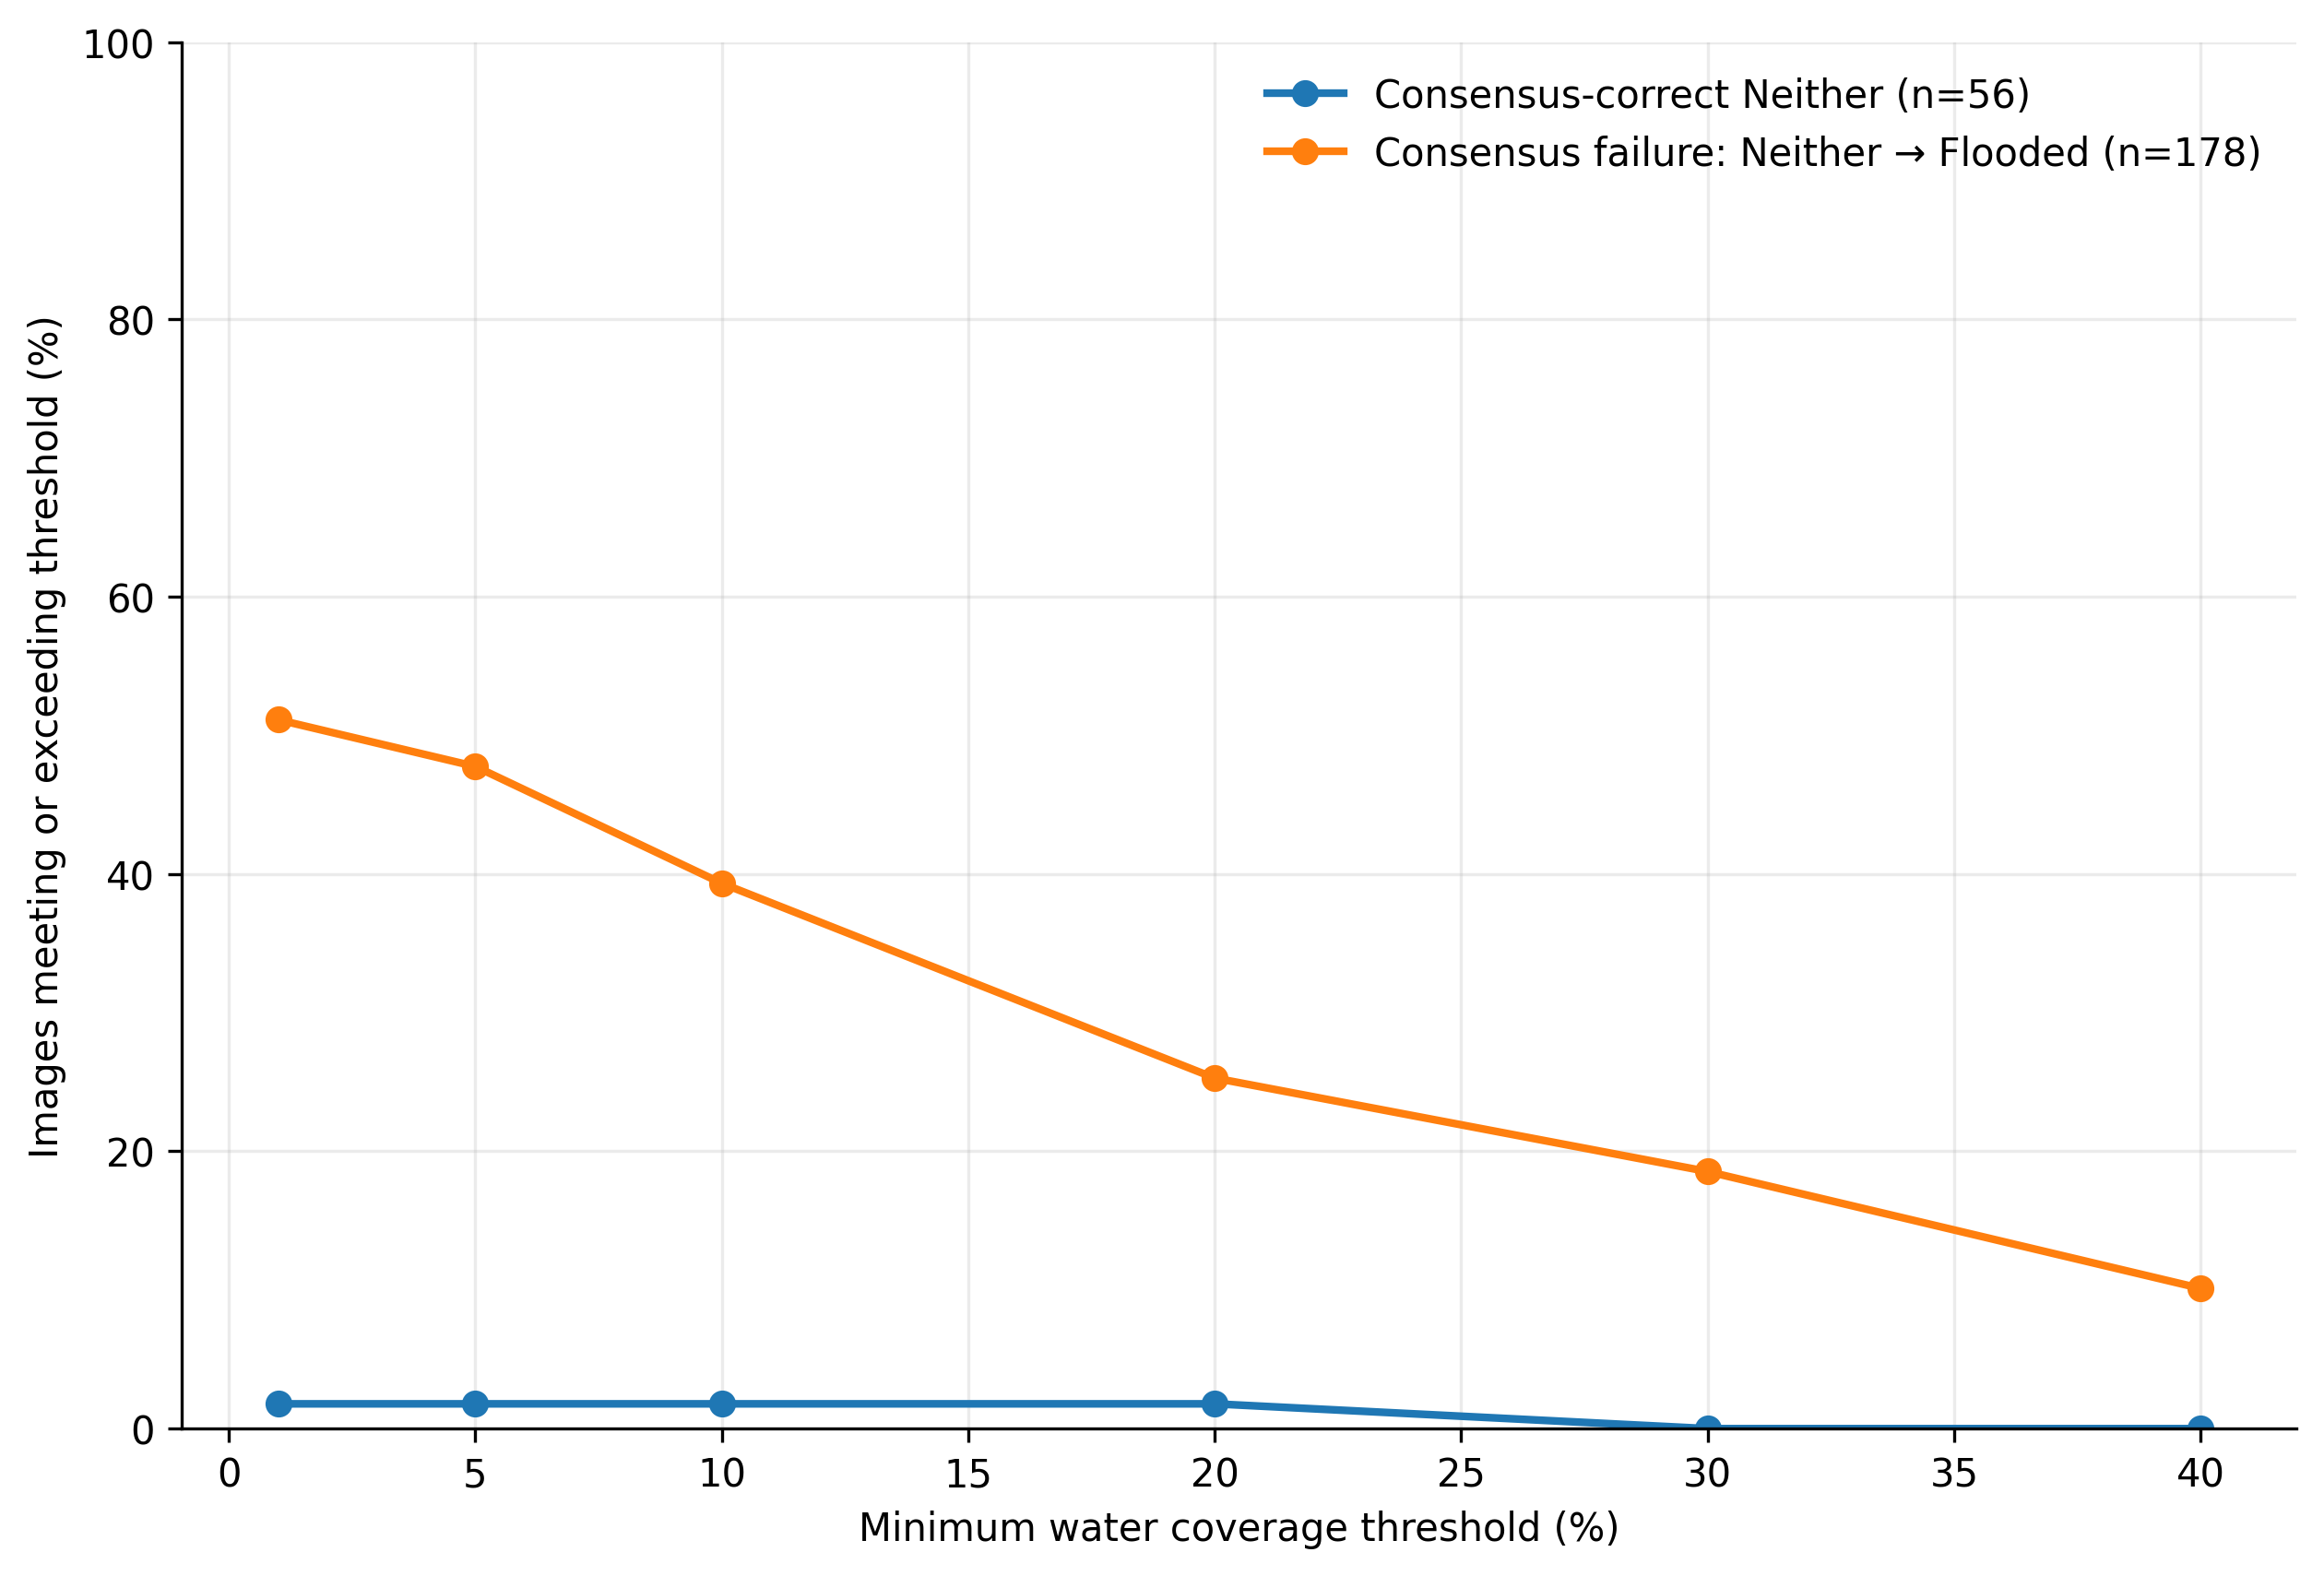
\includegraphics[width=\linewidth]
    {Fig_water_coverage_threshold_curve.png}

    \vspace{-1mm}
    \textbf{(c)}
\end{minipage}

\caption{
Post-hoc FloodNet segmentation analysis.
(a) Segmentation-class presence rates.
(b) Mean image area occupied by each segmentation class.
(c) Fraction of consensus-failure and consensus-correct Neither scenes
meeting increasingly strict Water-coverage thresholds.
Consensus false-flood scenes contain substantially more ordinary Water
and non-flooded Road context and are less strongly grass-dominated.
}
\label{fig:segmentation_triptych}
\end{figure*}

Taken together with the Grad-CAM observations, the segmentation
analysis is consistent with reliance on flood-associated contextual
cues, including ordinary water, non-flooded roads, and heterogeneous
terrain, rather than a complete semantic distinction between ordinary
water and true inundation.

Because the segmentation hypothesis was developed after observing the
external failure pattern, these results establish association rather
than causality.

% Ensure Results floats appear before Limitations.
\clearpage
